\documentclass{article}
\usepackage{graphicx} % Required for inserting images
\usepackage{booktabs} % For better table formatting
\usepackage{array}    % For more flexible table features
\usepackage{placeins} % To control figure placement
\usepackage{float}    % To use the H placement specifier

\title{Analysis of Single Mutants}
\author{Your Name} % Replace with your name
\date{}

% Set graphic path to the directory containing the images
\graphicspath{{/home/hp/nayanika/github/GPX6/figures/}} % Add the path to your images

\begin{document}

\maketitle

\section*{Introduction}
To guide the selection of mutations for directed evolution, a multiple sequence alignment was performed between the human and mouse wild-type protein. This MSA revealed 47 positions that differed between the human and mouse sequences, suggesting potential sites for mutagenesis. In order to prioritize residues for mutagenesis, the distances from the alpha carbon of Cys/Sec49 (active site residue) and the rest of the 46 positions were calculated. Residues were then grouped into distance criteria of <10 Å, 10-15 Å, 15-20 Å, 20-25 Å, 25-30 Å, and 30-35 Å. This distance-based approach allowed us to select residues within different proximity ranges to Cys/Sec49. Grouping residues into distance bins provides a systematic and stochastic way to explore the impact of mutations at varying distances from the target residue (Cys/Sec49). 

To investigate the individual contributions of each residue to the structural and functional differences between the human and mouse proteins, single mutants were generated systematically. Each mutation corresponds to substituting a residue in the mouse protein with its human counterpart, or vice versa, as outlined in the mutation table of 47 residues. This process was conducted one residue at a time to isolate the effects of each mutation.

The mutations were applied by transferring each residue from the mouse sequence to the human sequence and vice versa, ensuring a controlled and systematic approach to mutagenesis. The active site residue, Cys/Sec49, remained a fixed reference point, with all mutations being calculated relative to it. For example, residues such as position 3 (N to K) and position 4 (R to S) involved changes in side-chain polarity or charge, while others, such as position 48 (Y to F), focused on aromatic substitutions. These single-residue changes allow for direct comparisons of the energetic and structural effects of each mutation, enabling us to study how these variations influence activation barriers and overall protein function.

By analyzing the 47 single mutants, we aim to systematically explore the structural transitions and activation energy changes associated with the human-to-mouse and mouse-to-human sequence transformations. This stepwise approach ensures that the contributions of individual residues to protein evolution and function are thoroughly characterized.

\begin{figure}[H]
    \centering
    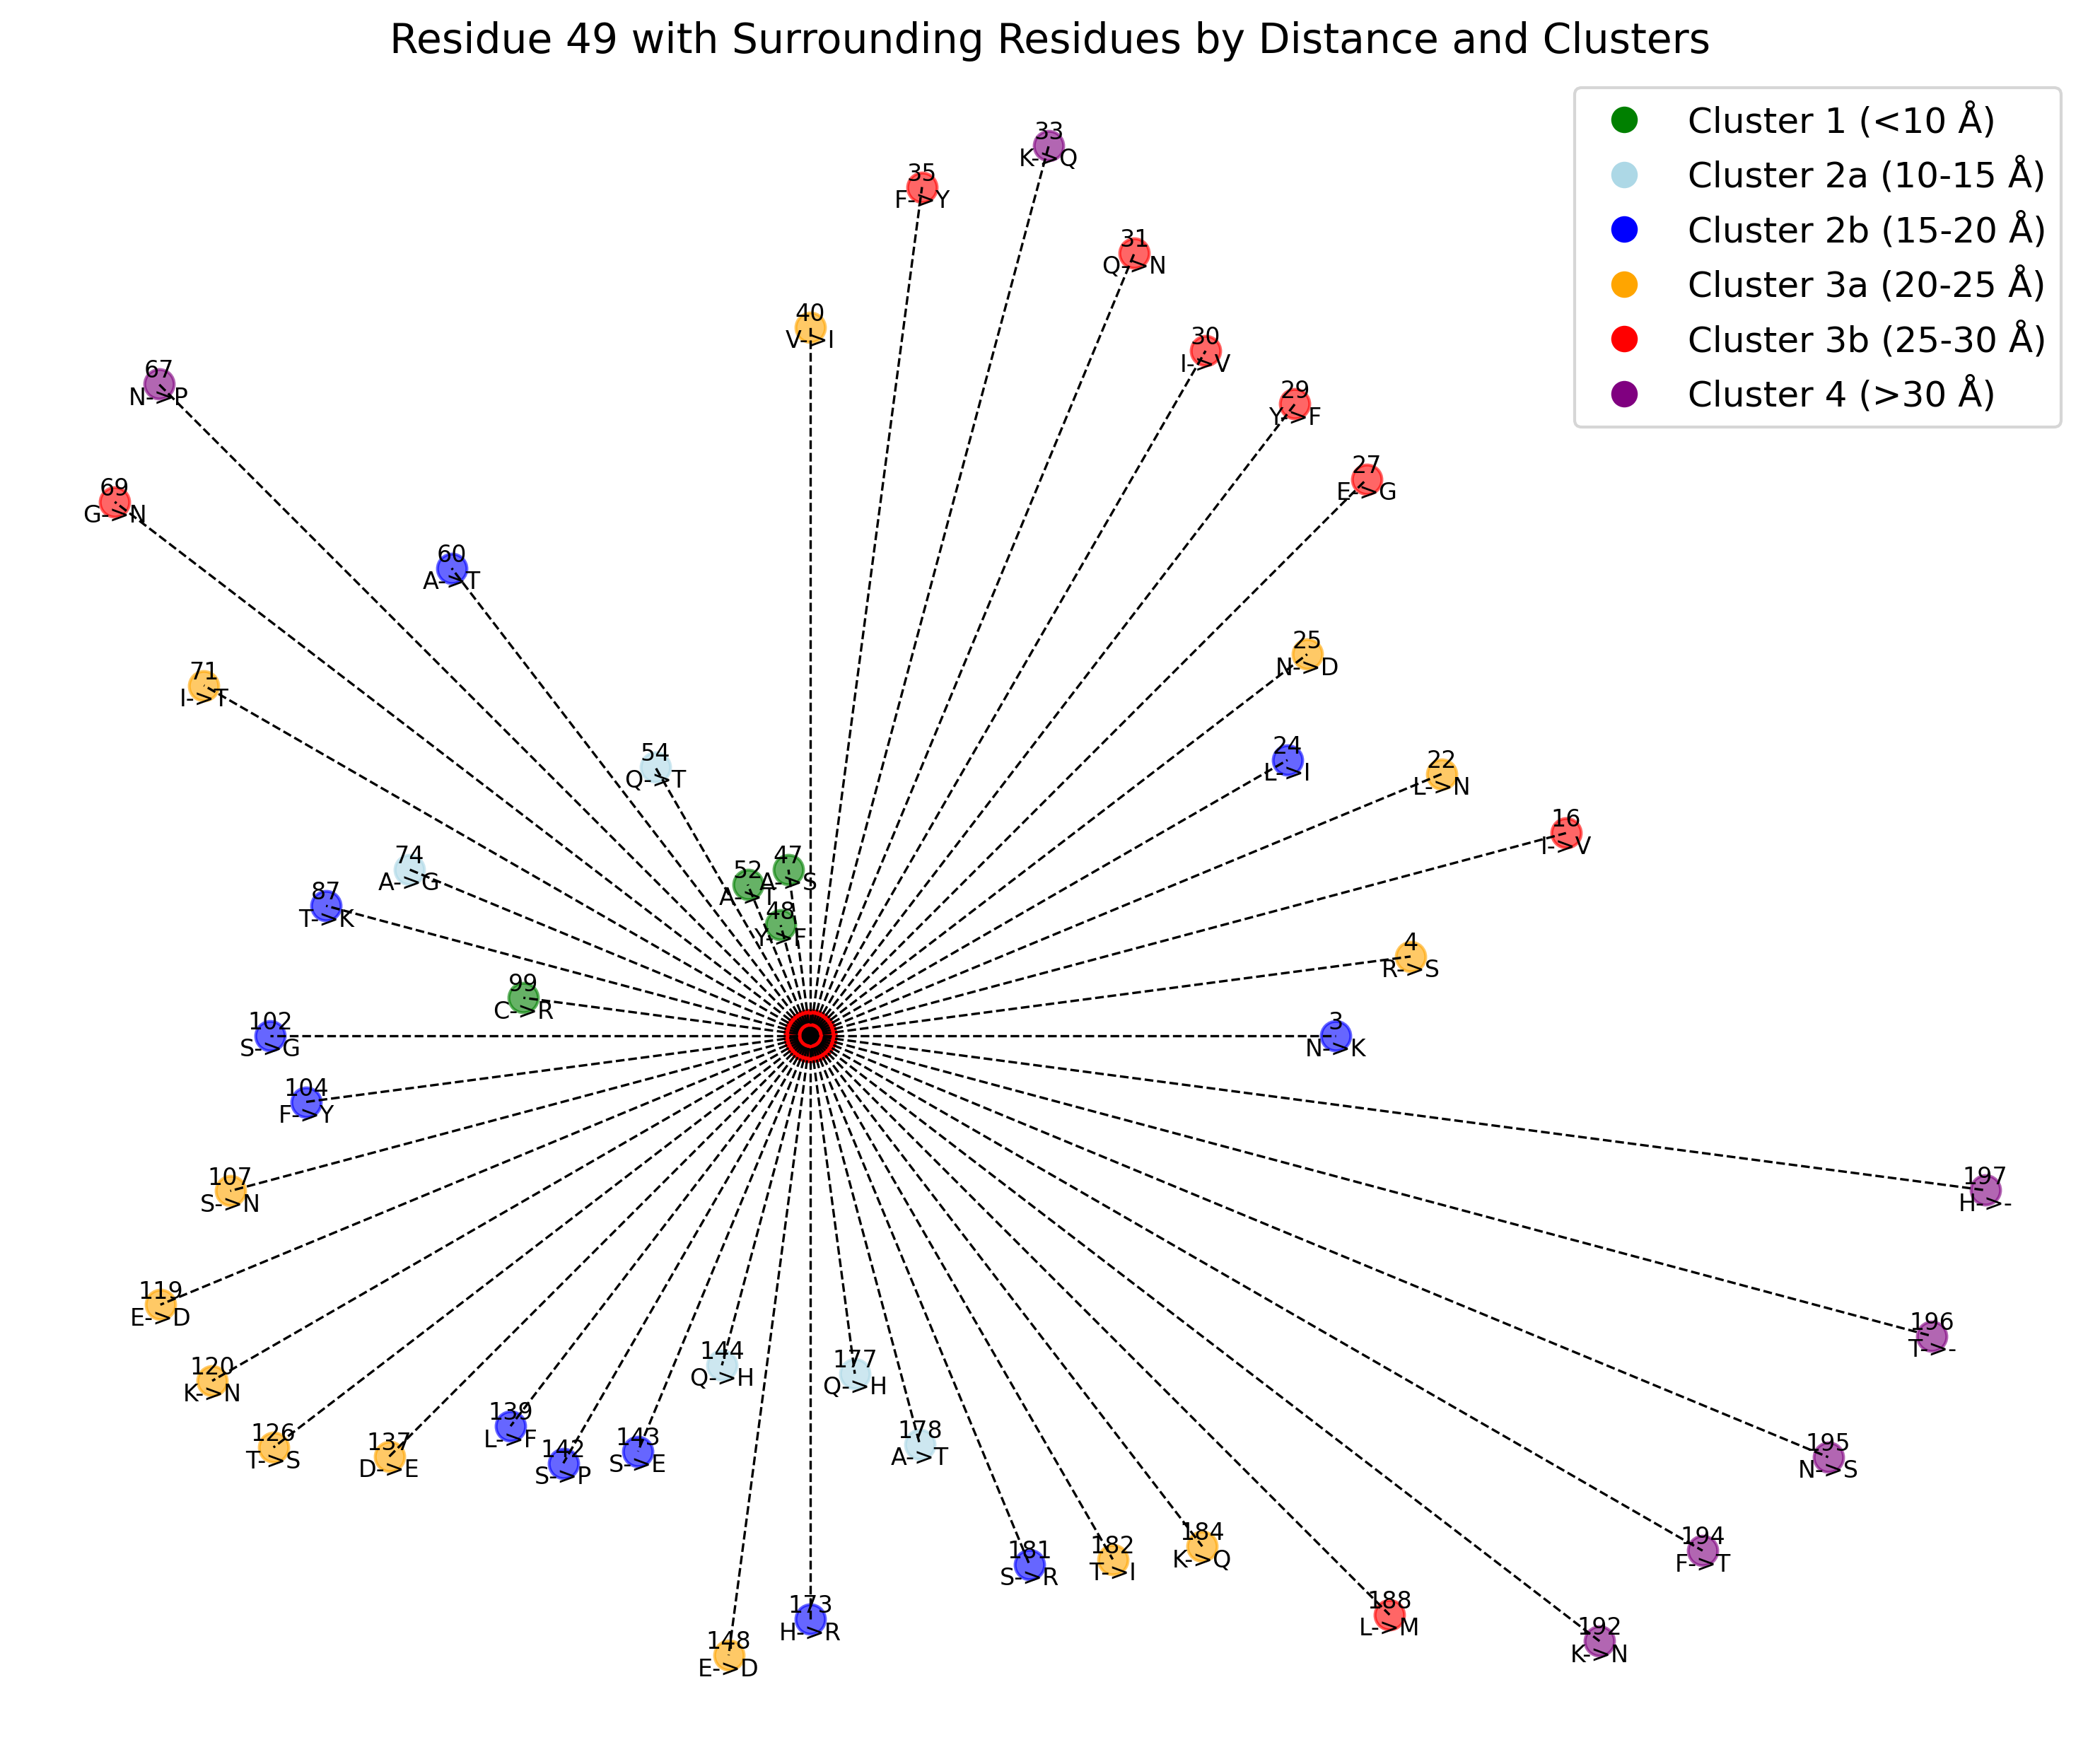
\includegraphics[width=0.8\linewidth]{Residue_human_Distances.png}
    \caption{Distance of residues from the active site for human mutants. The figure highlights proximity of each residue to Cys/Sec49.}
    \label{fig:human_distances}
\end{figure}

\begin{figure}[H]
    \centering
    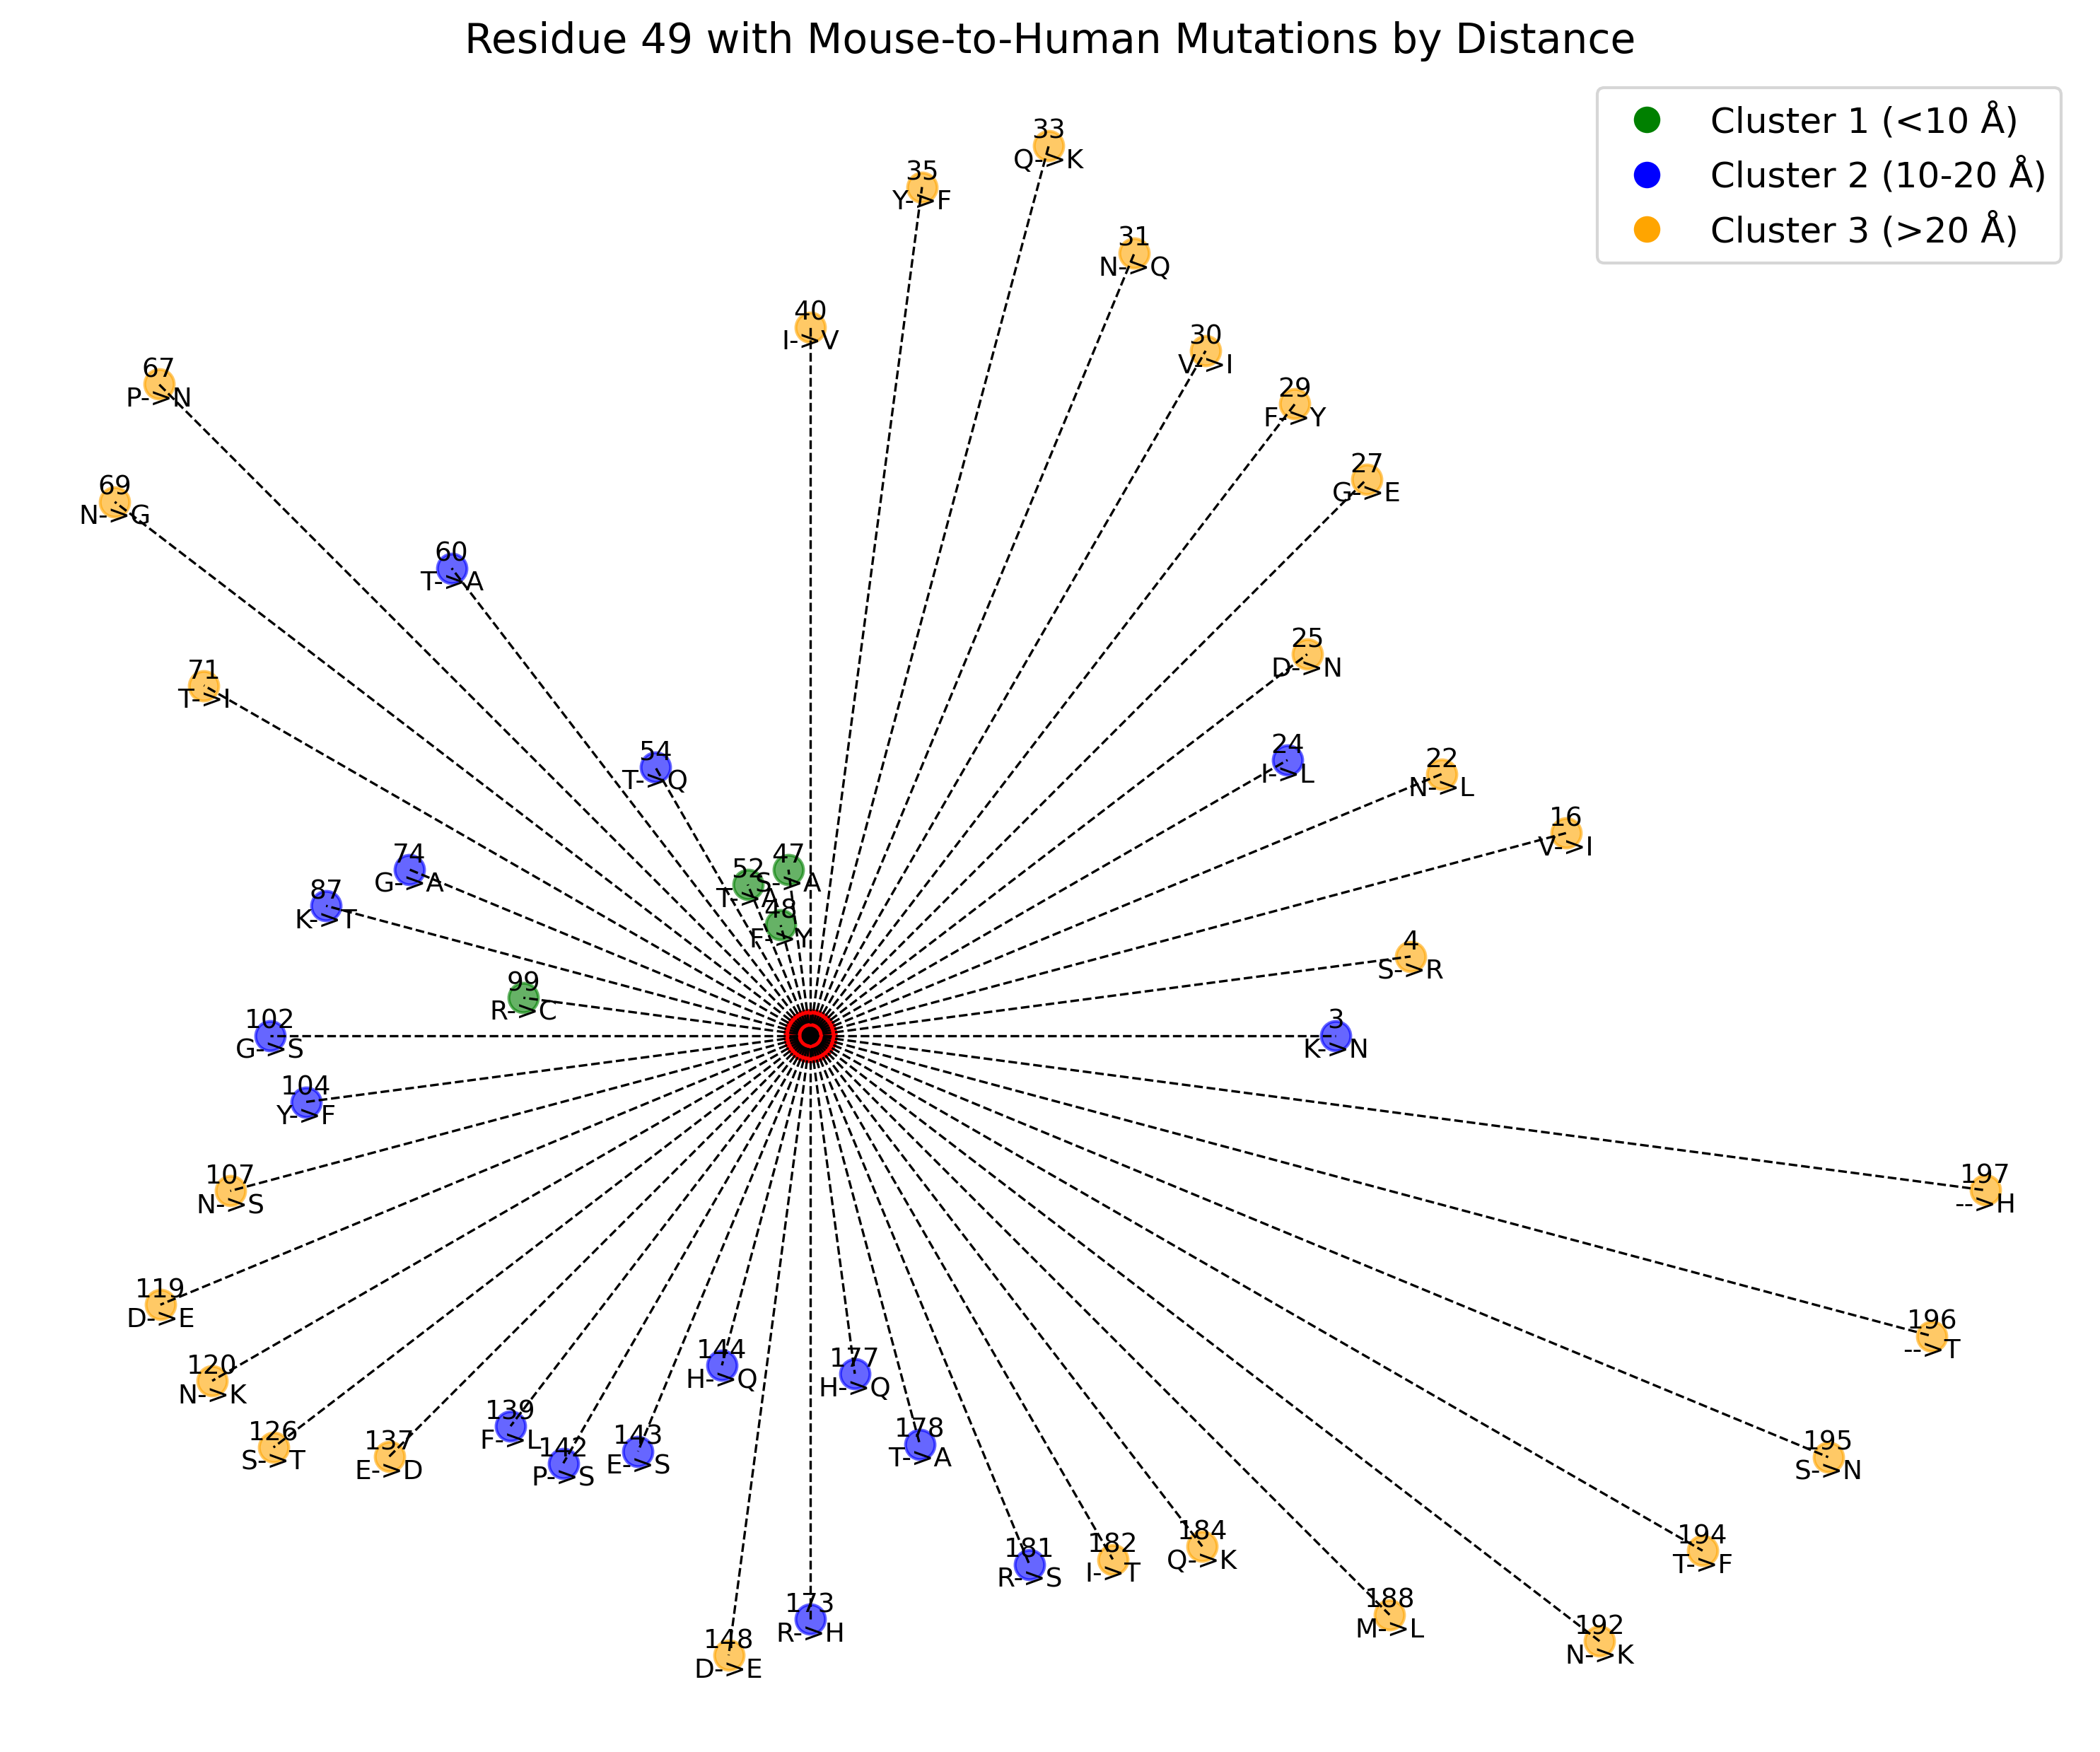
\includegraphics[width=0.8\linewidth]{Residue_mouse_Distances.png}
    \caption{Distance of residues from the active site for mouse mutants. The figure highlights proximity of each residue to Cys/Sec49.}
    \label{fig:mouse_distances}
\end{figure}

\FloatBarrier % Forces all previous figures to appear before this section

\subsection{Clustering the Variants}
The output explains the clustering results of the residues based on their coordinates, which are derived from their distance and free energy values. Here's what the output indicates:

Clusters:
\begin{itemize}
    \item \textbf{Cluster 1:} This cluster contains most of the residues, with coordinates generally clustered at higher distance and free energy values. For example, residues like 3 (Coordinates = (21.63, 24.64)) and 4 (Coordinates = (19.64, 22.52)) are in this cluster. Residues that belong to this cluster have relatively closer distances to each other in terms of both the distance and free energy values, with some exceptions for outliers like residues 33 and 192, which are farther from the cluster's centroid.
    \item \textbf{Cluster 2:} This cluster has a few residues that are grouped separately based on their distinct coordinate values. Examples include residue 24 (Coordinates = (18.69, 17.85)) and residue 47 (Coordinates = (5.59, 17.38)). These residues generally have lower or more varied values for both distance and free energy compared to Cluster 1.
\end{itemize}

Centroids: The centroids of the two clusters are the average points of all residues in each cluster. The distances to these centroids reflect how far each residue is from the center of its cluster. Residues closer to the centroid have a smaller distance, while those farther away are considered outliers or more variable. For example, Residue 30 (Coordinates = (26.67, 20.93)) is very close to its centroid in Cluster 1 (Distance to Centroid = 2.04). Residue 33 (Coordinates = (30.54, 30.57)) has a relatively larger distance to the centroid (Distance = 11.92), indicating it may be somewhat of an outlier or not as well aligned with the main cluster.

Interpretation: The clustering reveals two distinct groups of residues based on their distance and free energy characteristics. Cluster 1 contains residues that have higher free energy and distance values and are generally more tightly clustered around their centroid. Cluster 2 contains residues with lower distance and free energy values, and they are more spread out from their centroid.

Outliers: Some residues (like 33, 192, 194, 195) are farther from their respective centroids, suggesting they may behave differently from the majority in terms of their distance and free energy values.

Overall, this clustering indicates that the residues naturally group into two major clusters, with a few outliers in each cluster. The distances to the centroids highlight which residues are more strongly associated with their respective clusters and which are farther away, suggesting variability in their behavior.

\FloatBarrier % Forces all previous figures to appear before this section

\subsection{Visualizing the Clusters}

The following figure illustrates the clustering of mutants based on the distances from the active site and other relevant features. This visualization provides a clear representation of how mutations at different positions affect the protein’s structure and potential function.

\end{document}
